\documentclass[journal,12pt,twocolumn]{IEEEtran}

\usepackage{setspace}
\usepackage{gensymb}
\singlespacing
\usepackage[cmex10]{amsmath}

\usepackage{amsthm}
\usepackage{url}

\usepackage{mathrsfs}
\usepackage{txfonts}
\usepackage{stfloats}
\usepackage{bm}
\usepackage{cite}
\usepackage{cases}
\usepackage{subfig}
\usepackage{tasks}

\usepackage{longtable}
\usepackage{multirow}

\usepackage{amsthm}

\usepackage{enumitem}
\usepackage{mathtools}
\usepackage{steinmetz}
\usepackage{tikz}
\usepackage{circuitikz}
\usepackage{verbatim}
\usepackage{tfrupee}
\usepackage[breaklinks=true]{hyperref}
\usepackage{graphicx}
\usepackage{tkz-euclide}

\usetikzlibrary{calc,math}
\usepackage{listings}
    \usepackage{color}                                            %%
    \usepackage{array}                                            %%
    \usepackage{longtable}                                        %%
    \usepackage{calc}                                             %%
    \usepackage{multirow}                                         %%
    \usepackage{hhline}                                           %%
    \usepackage{ifthen}                                           %%
    \usepackage{lscape}     
\usepackage{multicol}
\usepackage{chngcntr}

\DeclareMathOperator*{\Res}{Res}

\renewcommand\thesection{\arabic{section}}
\renewcommand\thesubsection{\thesection.\arabic{subsection}}
\renewcommand\thesubsubsection{\thesubsection.\arabic{subsubsection}}

\renewcommand\thesectiondis{\arabic{section}}
\renewcommand\thesubsectiondis{\thesectiondis.\arabic{subsection}}
\renewcommand\thesubsubsectiondis{\thesubsectiondis.\arabic{sub subsection}}


\hyphenation{optical networks semiconduc-tor}
\def\inputGnumericTable{}                                 %%

\lstset{
%language=C,
frame=single, 
breaklines=true,
columns=fullflexible
}
\date{March 2021}

\begin{document}

\newcommand{\BEQA}{\begin{eqnarray}}
\newcommand{\EEQA}{\end{eqnarray}}
\newcommand{\define}{\stackrel{\triangle}{=}}
\bibliographystyle{IEEEtran}
\raggedbottom
\setlength{\parindent}{0pt}
\providecommand{\mbf}{\mathbf}
\providecommand{\pr}[1]{\ensuremath{\Pr\left(#1\right)}}
\providecommand{\qfunc}[1]{\ensuremath{Q\left(#1\right)}}
\providecommand{\fn}[1]{\ensuremath{f\left(#1\right)}}
\providecommand{\e}[1]{\ensuremath{E\left(#1\right)}}
\providecommand{\sbrak}[1]{\ensuremath{{}\left[#1\right]}}
\providecommand{\lsbrak}[1]{\ensuremath{{}\left[#1\right.}}
\providecommand{\rsbrak}[1]{\ensuremath{{}\left.#1\right]}}
\providecommand{\brak}[1]{\ensuremath{\left(#1\right)}}
\providecommand{\lbrak}[1]{\ensuremath{\left(#1\right.}}
\providecommand{\rbrak}[1]{\ensuremath{\left.#1\right)}}
\providecommand{\cbrak}[1]{\ensuremath{\left\{#1\right\}}}
\providecommand{\lcbrak}[1]{\ensuremath{\left\{#1\right.}}
\providecommand{\rcbrak}[1]{\ensuremath{\left.#1\right\}}}
\theoremstyle{remark}
\newtheorem{rem}{Remark}
\newcommand{\sgn}{\mathop{\mathrm{sgn}}}
\providecommand{\abs}[1]{\vert#1\vert}
\providecommand{\res}[1]{\Res\displaylimits_{#1}} 
\providecommand{\norm}[1]{\lVert#1\rVert}
%\providecommand{\norm}[1]{\lVert#1\rVert}
\providecommand{\mtx}[1]{\mathbf{#1}}
\providecommand{\mean}[1]{E[ #1 ]}
\providecommand{\fourier}{\overset{\mathcal{F}}{ \rightleftharpoons}}
%\providecommand{\hilbert}{\overset{\mathcal{H}}{ \rightleftharpoons}}
\providecommand{\system}{\overset{\mathcal{H}}{ \longleftrightarrow}}
	%\newcommand{\solution}[2]{\textbf{Solution:}{#1}}
\newcommand{\solution}{\noindent \textbf{Solution: }}
\newcommand{\cosec}{\,\text{cosec}\,}
\providecommand{\dec}[2]{\ensuremath{\overset{#1}{\underset{#2}{\gtrless}}}}
\newcommand{\myvec}[1]{\ensuremath{\begin{pmatrix}#1\end{pmatrix}}}
\newcommand{\mydet}[1]{\ensuremath{\begin{vmatrix}#1\end{vmatrix}}}
\numberwithin{equation}{subsection}
\makeatletter
\vspace{3cm}
\title{Assignment 4}
\author{Suraj - CS20BTECH11050}
\maketitle
\newpage
\bigskip
\renewcommand{\thetable}{\theenumi}
\newcommand{\dsum}{\displaystyle\sum}
\newcommand{\comb}[2]{{}^{#1}\mathrm{C}_{#2}}
\newcommand{\R}{\mathbb{R}}
\newcommand{\C}{\mathbb{C}}
\newcommand{\Int}{\int\limits}
\newtheorem{theorem}{Theorem}[section]
Download all python codes from 
\begin{lstlisting}
https://github.com/Suraj11050/Assignments-AI1103/tree/main/Assignment%204/Python%20codes
\end{lstlisting}
%https://www.overleaf.com/project/604c4c718ee4e22400cf9d22
Download Latex-tikz codes from 
%
\begin{lstlisting}
https://github.com/Suraj11050/Assignments-AI1103/blob/main/Assignment%204/Assignment%204.tex
\end{lstlisting}
\section{GATE 2021 (ST), Q.17 (STATISTICS SECTION)} 
If the marginal probability density function of the $k^{th}$ order statistic of a 
random sample of size 8 from a uniform distribution on $[0,2]$ is
\[
  f(x) =
  \begin{cases}
   \dfrac{7}{32}\,x^{6}\,\brak{2-x},  & 0<x<2, \\ 
      \hspace{1cm}   0,               & \text{otherwise,} 
  \end{cases}
\]
then $k$ equals \underline{\hspace{3cm}}
\bigskip
\section{SOLUTION}
\textbf{Method 1:} \\
Let $X\in[0,2]$ be a random variable of uniform order statistic distribution of sample size 8 then
\begin{align}
 \int_{0}^{2} \pr{x}\,dx &= 1 \\
 \pr{x}                  &= \dfrac{1}{2}\;\brak{\because \text{Uniform order}}
\end{align}
The PDF for X is 
\begin{align}
\fn{x} = 
 \begin{cases}
  \dfrac{1}{2},      &0<x<2, \\ 
     0, &\text{otherwise,}
 \end{cases} \label{d}
\end{align}
 The CDF for X is 
 
 \begin{align}
 F(x) = 
 \begin{cases}
      0,             &x \leq 0, \\ 
  \dfrac{x}{2},      &0 < x< 2, \\ 
     1,              & x>2
 \end{cases} \label{e}
 \end{align}
 \begin{theorem}
Let $\{X_1, X_2, \cdots X_n\}$ be n i.i.d random variables with common CDF $= F(x)$ and common PDF $= f(x)$, 
then the marginal probability density of $k^{th}$ order statistic (PDF) is denoted by $f_{(k,n)}(x)$  and it
is given by
\begin{align}
f_{(k,n)}(x) = n\;\comb{n-1}{k-1}\,f(x)\,(F(x))^{k-1}\,\brak{1-F(x)}^{n-k} \label{eqn_2}
\end{align}
\end{theorem}
PDF of $k^{th}$ order statistic of given sample from equation \eqref{eqn_2}
\begin{align}
f_{(k,n)}(x) &= n\;\comb{n-1}{k-1}\,\dfrac{1}{2}\,\brak{\dfrac{x}{2}}^{k-1}\,\brak{1-\dfrac{x}{2}}^{n-k} \\
f_{(k,8)}(x) &= \dfrac{8}{2^{(1+(k-1)+(8-k))}}\times\comb{7}{k-1}\,x^{k-1}\,\brak{2-x}^{8-k}\\
f_{(k,8)}(x) &= \comb{7}{k-1}\,\dfrac{1}{32}\,x^{k-1}\,\brak{2-x}^{8-k} \label{c}
 \end{align}
Comparing the PDF obtained in equation \eqref{c} with the equation given in question
\begin{align}
\dfrac{1}{32}\,\comb{7}{k-1}\,\brak{2-x}^{8-k}\,x^{k-1} &= \dfrac{7}{32}\,\brak{2-x}\,x^6 \\
\therefore k &= 7 
\end{align}
Hence the marginal probability density given is $7^{th}$ order statistic and 
\textbf{the value of k is 7}
\null \par \null
\textbf{Method 2:}\\
we know that, PDF of $k^{th}$ order statistic of a uniform distribution on $[0,1]$ follows 
beta distribution
\begin{align}
\Int_{0}^{2}f(x)\,dx &= \Int_{0}^{2} \dfrac{7}{32}\,x^{6}\,\brak{2-x}\,dx \\
\Int_{0}^{2}f(x)\,dx &= \Int_{0}^{2} 56\,\brak{\dfrac{x}{2}}^{6}\,\brak{1-\dfrac{x}{2}}\,d\brak{\dfrac{x}{2}}
\end{align}
Let new random variable be $t$ such that $t=x/2$, New sample be $\{T_1,\cdots T_8\}$ such that $T_{i}=X_{i}/2$.

\newpage

\begin{align}
f(t) &= 56\,t^{6}\,\brak{1-t} \\
\Int_{0}^{2}f(x)\,dx &=  \Int_{0}^{1}f(t)\,dt = 1
\end{align}
The Uniform distribution of new random sample is on $[0,1]$ such that   PDF $= 1$ and CDF $= t$ \\
Given $k^{th}$ order statistic (after conversion)
\begin{align}
f_{(k,8)}(t) =
  \begin{cases}
      56\,t^{6}\,\brak{1-t},  & 0<t<1, \\ 
      \hspace{1cm}   0,               & \text{otherwise,} 
  \end{cases}
  \label{pdf_t}
\end{align}
Since equation \eqref{pdf_t} is a Beta distribution with $r=k$, $s=n-k+1$  
\begin{align}
r-1 = k-1 &= 6 \\
\therefore k &= 7 
\end{align}
Hence the \textbf{value of k is 7}
\null \par \null
\textbf{Presentation link :} 
\null \par
\url{https://github.com/Suraj11050/Assignments-AI1103/tree/main/Assignment 4 presentation}

\newpage

\begin{figure}[htp]
    \centering
    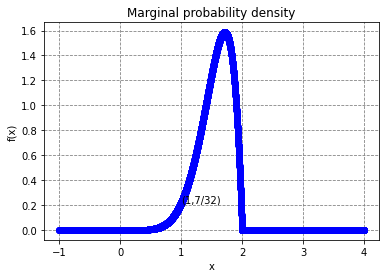
\includegraphics[width = \columnwidth]{MPD_1.png}
    \label{fig:maginal probability density 1}
    \caption{PDF of $f_{(7,8)}(x)$}
\centering
    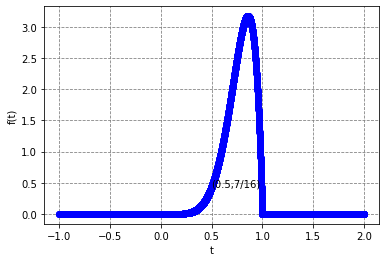
\includegraphics[width = \columnwidth]{MPD_2.png}
    \label{fig:maginal probability density 2}
    \caption{PDF of $f_{(7,8)}(t)$}
\end{figure}
\end{document}
